\chapter{Metodologia}
Com o intuito de guiar a pesquisa de forma adequada, esse capítulo aborda sobre os diversos tipos de metodologias de pesquisa, de modo a definir qual se adequa melhor ao projeto. Este capítulo traz também a modelagem da metodologia de pesquisa que será utilizada, além do cronograma da pesquisa e a prova de conceito.

\section{Classificação da pesquisa}
	As pesquisas podem ser classificadas quanto ao seus objetivos gerais ou quanto aos procedimentos técnicos utilizados. A classificação das pesquisas quanto aos seus objetivos gerais é muito importante para estabelecer uma visão teórica, ou seja, possibilitar uma aproximação conceitual. Porém, é necessário confrontar essa visão teórica com dados realistas, fornecendo uma visão empírica. Desta forma, faz-se necessário traçar um modelo conceitual e operativo, chamado delineamento, e que tem como parte mais importante a definição do procedimento que será utilizado na coleta de dados. Logo, as pesquisas podem ser classificadas de acordo com seu delineamento, ou seja, quanto aos procedimentos técnicos utilizados \cite{ac2002elaborar}.

\subsection{Quanto aos objetivos gerais}
	As pesquisas classificadas pelos objetivos gerais podem ser divididas em 3 (três) grandes grupos: pesquisas exploratórias, pesquisas descritivas e pesquisas explicativas \cite{ac2002elaborar}. Cada um desses grupos será detalhado nas subseções a seguir apresentadas. 
\subsubsection{Pesquisa exploratória}
	A pesquisa exploratória tem um caráter investigativo sobre um assunto pouco conhecido. Tem por objetivo facilitar a delimitação do tema de pesquisa através de informações proporcionadas pela exploração \cite{prodanov2013metodologia}. Por isso, seu planejamento é bastante flexível, de modo que considere os mais diversos aspectos acerca do tema estudado. Em grande maioria, as pesquisas exploratórias assumem a forma de pesquisa bibliográfica ou estudo de caso, envolvendo levantamento bibliográfico, entrevistas com pessoas que tiveram experiências práticas com o problema pesquisado e/ou análise de exemplos que estimulem a compreensão \cite{ac2002elaborar}.
\subsubsection{Pesquisa descritiva}
	Na pesquisa descritiva, o pesquisador apenas observa, registra, analisa e ordena os dados dos fatos observados sem interferir de forma alguma no processo. Envolve o uso padronizado de coleta de dados podendo ser questionário e/ou observação sistemática. Em geral, assume a forma de levantamento \cite{ac2002elaborar}. 
A pesquisa descritiva tem por objetivo descrever as características de determinada população, fenômeno ou estabelecimento de relações entre variáveis procurando classificar, explicar e interpretar os fatos que ocorrem, diferindo da pesquisa experimental que pretende demonstrar o modo ou as causas de um dado fato ocorrido \cite{prodanov2013metodologia}.
\subsubsection{Pesquisa explicativa}
	A pesquisa explicativa, assim como o nome sugere, busca explicar os motivos pelos quais ocorrem os fatos observados, por meio do registro, análise, classificação e interpretação dos fenômenos observados. 
Em geral, quando realizada nas ciências naturais, requer o uso do método experimental que possibilita a manipulação e controle de variáveis, e quando realizada nas ciências sociais, requer o uso do método observacional. Dessa forma, a pesquisa explicativa assume a forma de pesquisa experimental ou pesquisa \textit{ex-post facto}. \cite{prodanov2013metodologia}

\subsection{Quanto aos procedimentos}
	As pesquisas classificadas quanto aos procedimentos técnicos utilizados podem ser divididas em 2 (dois) grupos: pesquisas que se valem das fontes de "papel", sendo elas classificadas em bibliográfica ou documental; e as pesquisas cujos dados são fornecidos por pessoas, sendo classificadas em experimental, \textit{ex-post facto}, levantamento ou estudo de caso \cite{ac2002elaborar}. Cada uma dessas classificações será detalhada a seguir.

\subsubsection{Pesquisa bibliográfica} 
	Uma pesquisa bibliográfica é desenvolvida exclusivamente a partir de fontes bibliográficas, principalmente de livros e artigos científicos. As fontes bibliográfcas podem ser classificadas de acordo com a Figura \ref{tiposDePesquisaBibliografica}.

\begin{figure}[h]
\centering
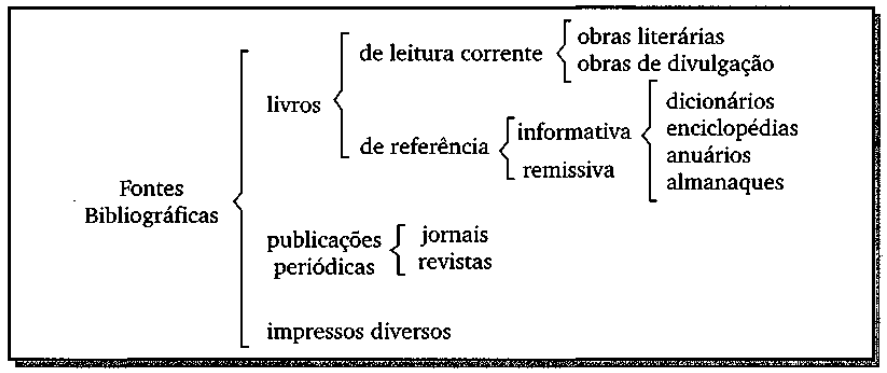
\includegraphics[keepaspectratio=true,scale=0.3]{figuras/tiposDePesquisaBibliografica.png}
\caption{Classificação das pesquisas bibliográficas \cite{ac2002elaborar}}
\label{tiposDePesquisaBibliografica}
\end{figure}
	
	Os livros são fontes bibliográficas de excelência, classificados como de leitura corrente ou de referência. Os livros de literatura corrente são aqueles que objetivam conferir conhecimentos científicos ou técnicos ao leitor, já os de referência tem por objetivo proporcionar ao leitor a rápida obtenção das informações requeridas (informativa) ou a referência às obras que as contenham (remissiva) \cite{ac2002elaborar}.  
A pesquisa bibliográfica é muito vantajosa ao pesquisador, já que este pode ter acesso a uma gama de informações muito maior do que aquelas que ele conseguiria pesquisando diretamente. Essa pesquisa também é de suma importância nas pesquisas históricas, pois a maioria dos fatos só é possível conhecer por esse tipo de pesquisa.
A desvantagem dessa pesquisa é a possível propagação de erros, pois se a fonte bibliográfica utilizada estiver com algum dado equivocado, este será refletido no trabalho do pesquisador.	
\subsubsection{Pesquisa documental}
	A pesquisa documental é difícil de distinguir da pesquisa bibliográfica, pois ambas utilizam material impresso para um determinado público como fonte de pesquisa. A principal diferença que se pode destacar é quanto ao tratamento análitico das fontes. A pesquisa documental utiliza fontes de pesquisa que não passaram por um tratamento análitico, ou seja, são matéria-prima como cartas pessoais, fotos, diários, memorandos e outros, a partir da qual o pesquisador vai desenvolver a sua pesquisa. A pesquisa bibliográfica se utiliza de fontes de pesquisa já analisadas como livros e periódicos \cite{ac2002elaborar}.
\subsubsection{Pesquisa experimental}
	A pesquisa experimental consiste em determinar o objeto de estudo, as possíveis variáveis capazes de influenciá-lo, as formas de controle e observação dos efeitos, fazendo com que o pesquisador seja o agente ativo da pesquisa. Uma pesquisa experimental pode ser desevolvida em qualquer lugar, desde que ela possa ser manipulada e controlada pelo pesquisador e que haja uma distribuição aleatória dos elementos que irão participar do experimento. As pesquisas experimentais são as mais utilizadas para se provar hipóteses de causa-efeito, porém é um ambiente com variáveis controladas, logo, pode haver variáveis de controle difícil ou até mesmo impossível, tornando o experimento inviável. \cite{ac2002elaborar}
\subsubsection{Pesquisa \textit{ex-post facto}}
	A tradução literal de \textit{ex-post facto} é "de um fato passado", ou seja, a pesquisa \textit{ex-post facto} é realizada após a ocorrência de variáveis no objeto de estudo. A diferença entre a pesquisa \textit{ex-post facto} e a pesquisa experimental é que esta verifica a causa-efeito com o controle de variáveis, enquanto aquela verifica a causa-efeito sem o controle de variáveis, já que o fato já ocorreu. Esse tipo de pesquisa é muitas vezes chamada de correlacional, pois nela é possível se identificar a existência de relação entre variáveis. \cite{ac2002elaborar}
\subsubsection{Levantamento}
	O levantamento é utilizado quando se interroga diretamente as pessoas que se quer conhecer o comportamento, procura ser representativo de universo definido, identificando as características dos componentes desse universo e oferecendo resultados pela precisão estática, através da caracterização dos segmentos. Um questionário pode ser utilizado para coletar os dados, e depois é feita a análise quantitativa dessa coleta. Quando um levantamento é feito sobre um grupo muito grande de pessoas, este é chamado de "censo". \cite{prodanov2013metodologia} 	
\subsubsection{Estudo de caso}
		O estudo de caso busca o aprofundamento nas questões propostas, estudando um único grupo ou comunidade, utilizando mais a observação direta do que a interrogação, captando as explicações e interpretações do que ocorre no grupo. No estudo de campo, o pesquisador está inserido no grupo, para poder entender melhor as regras, os costumes e as convenções.

\section{Planejamento da pesquisa}
	O modelo híbrido de pesquisa exploratório/experimental será utilizado nesse TCC para avaliar os vários tipos de algoritmos que podem ser utilizados como solução para a questão de pesquisa. Após a escolha do algoritmo ter sido feita, este será adaptado ao contexto do LEGO Mindstorms, utilizando o modelo híbrido de pesquisa exploratório/descritivo.
Pretende-se ainda, nas atividades específicas de desenvolvimento, fazer uso de uma  metodologia orientada aos princípios ágeis, uma possível adaptação do Scrum, com sprints
de uma semana (em média), as quais ocorrerão em ambiente controlado e terão seus resultados quantificados.
	Dado que a pesquisa será exploratória/experimental e exploratória/descritiva, muito provavelmente será utilizado o modelo de pesquisa-ação ao longo do projeto. Esse modelo permitirá, dentre outras contribuições, a retroalimentação da solução com base nos experimentos realizados ao longo da condução do trabalho.

\section{Modelagem da metodologia}
	A modelagem da metodologia utilizada neste trabalho demonstra, de forma clara, o fluxo das atividades tanto do trabalho de conclusão de curso 1 quanto do trabalho de conclusão de curso 2, visto que um é a continuação do outro.

Inicialmente foi realizado um levantamento bibliográfico preliminar sobre robótica, algoritmos de otimização, como o algoritmo guloso, e programação dinâmica, a fim de dar suporte à definição do escopo do projeto. A seguir, foi realizado um planejamento da abordagem para definir se a mesma seria ou não viável. Após a aprovação do escopo, foi definido um referencial teórico, um suporte tecnólogico e uma metodologia de pesquisa. Concluídos esses passos, foi elaborada a prova de conceito onde buscou-se avaliar a viabilidade da proposta, abordando a integração do robô com a linguagem Prolog, e uma avaliação dos algoritmos de otimização (algoritmo guloso e programação dinâmica), vide seção \ref{provaDeConceito}. Em seguida, foi elaborada a parte escrita da proposta. 

A apresentação para a banca avaliadora findará a fase do TCC 01, dando início ao TCC 02. Este começa com a coleta e realização das sugestões de melhoria feitas pela banca avaliadora, a seguir serão definidos cenários de uso que para serem utilizados na avaliação dos resultados da implementação da máquina de raciocínio. 
A \textit{First Lego League} utiliza em cada torneio um tapete de missões diferente. Para a criação de cada cenário de uso, será utilizado um tapete diferente, e cada tapete contêm  missões diferentes. O primeiro cenário de uso será utilizando o tapete de missões \textit{Nature's Fury}, vide seção \ref{tapeteDeMissoes}, e o ideal será a máquina de raciocínio contemplar no mínimo 3 cenários de uso.
Em \textit{sprints} de uma semana, durante três meses, a máquina de raciocínio será desenvolvida. A cada duas \textit{sprints}, uma \textit{release}, a máquina de raciocínio será testada no robô e seus resultados serão avaliados de acordo com os cenários de uso anteriormente definidos. Caso o resultado não seja satisfatório, uma nova \textit{release} será necessária. Quando a avaliação dos resultados for satisfatória (ou seja, os objetivos geral e específicos do TCC forem atingidos), será elaborada a parte escrita do projeto.

A definição temporal de uma \textit{release} ter duas \textit{sprints} e cada \textit{sprint} ter duas semanas é uma média, podendo haver \textit{sprints} ou \textit{releases} maiores ou menores, de acordo com a necessidade. Uma \textit{release} é dada por encerrada quando o código é testado no robô e seus resultados são avaliados. 

Com intuito de ilustrar como será realizada a condução deste projeto, segue a
Figura \ref{modelagem} que apresenta a modelagem do processo metodológico com base na metodologia descrita nesta seção.

\FloatBarrier
\begin{figure}[!h]
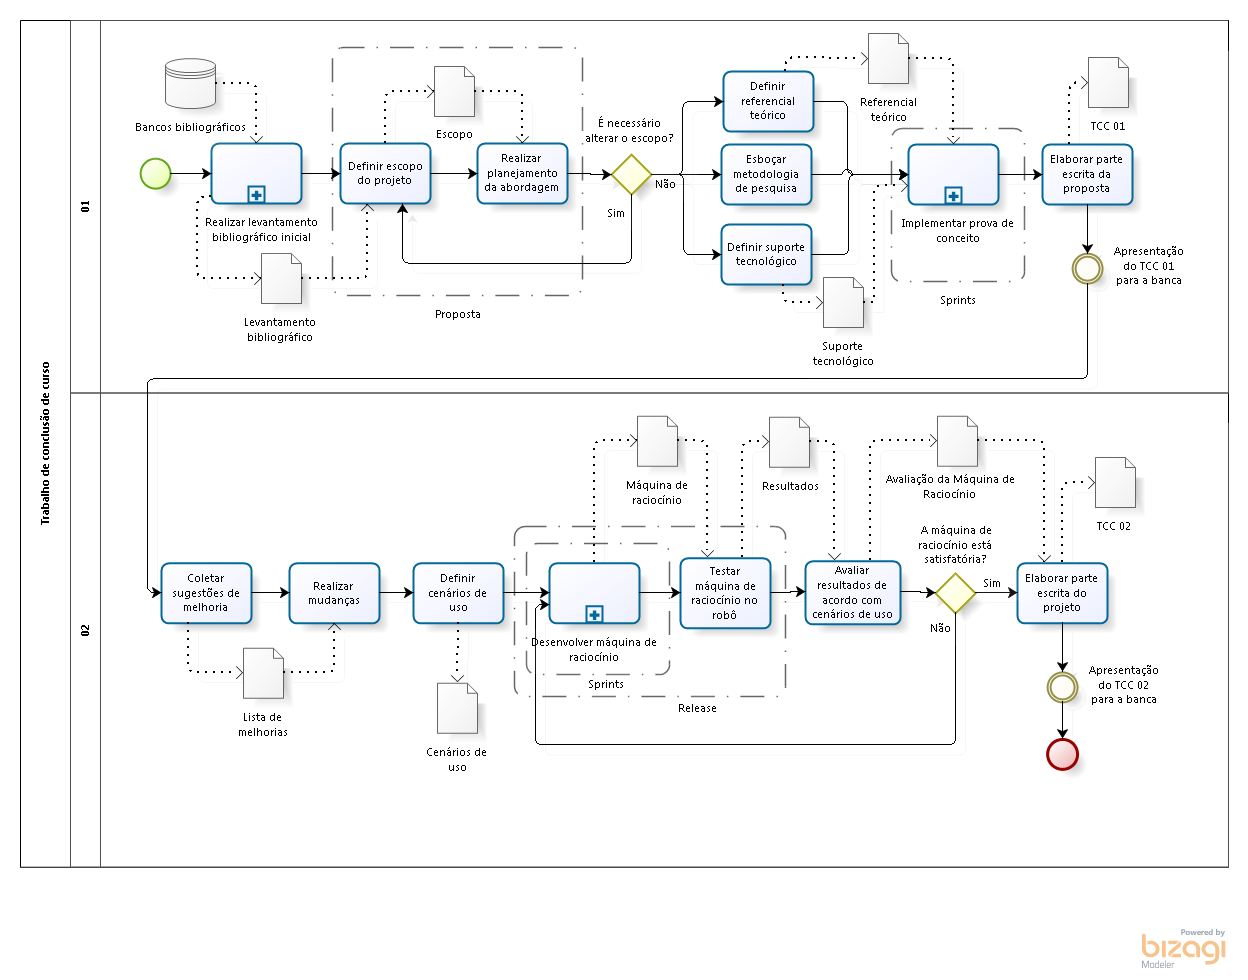
\includegraphics[keepaspectratio=true,scale=0.54]{figuras/modelagemTcc.png}
\caption{Modelagem do processo utilizado no TCC}
\label{modelagem}
\end{figure}
\clearpage
 
\section{Cronograma da pesquisa}
O cronograma, detalhado nas Tabelas \ref{tab01} e \ref{tab02}, visa conferir uma noção temporal acerca das atividades definidas para o processo. Trata-se de uma visão preliminar, logo, pode haver modificações ao longo do projeto de acordo com as necessidades.      

\FloatBarrier
\begin{table}[h]
	\centering
	
	\begin{tabular}{lcccccc}
		\toprule
		& \textbf{Jan} & \textbf{Fev} & \textbf{Mar} & \textbf{Abr} & \textbf{Mai} & 		
		\textbf{Jun} \\
		\midrule
		Realizar levantamento bibliográfico inicial & X & X &  &  &  &  \\
		\midrule
		Definir escopo do projeto &  & X &  &  &  &  \\
		\midrule
		Realizar planejamento da abordagem &  &  & X &  &  &  \\
		\midrule
		Definir referencial teórico &  &  &  & X & X &  \\
		\midrule
		Definir suporte tecnológico &  &  &  & X & X &  \\
		\midrule
		Esboçar metodologia de pesquisa &  &  &  & X & X &  \\
		\midrule
		Elaborar prova de conceito &  &  &  &  &  & X \\
		\midrule
		Elaborar parte escrita da proposta &  &  &  &  &  & X \\
		\bottomrule
	\end{tabular}

	\caption{Cronograma do TCC 01}
	\label{tab01}
\end{table}

\FloatBarrier
\begin{table}[h]
	\centering
	
	\begin{tabular}{lcccccc}
		\toprule
		& \textbf{Jul} & \textbf{Ago} & \textbf{Set} & \textbf{Out} & \textbf{Nov} & 		
		\textbf{Dez} \\
		\midrule
		Coletar sugestões de melhoria & X &  &  &  &  &  \\
		\midrule
		Realizar mudanças & X &  &  &  &  &  \\
		\midrule
		Definir cenários de uso & X &  &  &  &  &  \\
		\midrule
		Desenvolver máquina de racionício &  & X & X & X &  &  \\
		\midrule
		Testar máquina de raciocínio no robô &  &  & X & X &  &  \\
		\midrule
		Avaliar resultados de acordo com cenários de uso &  &  & X & X &  &  \\
		\midrule
		Elaborar parte escrita do projeto &  &  &  &  & X &  \\
		\bottomrule
	\end{tabular}

	\caption{Cronograma do TCC 02}
	\label{tab02}
\end{table}

\section{Prova de conceito} \label{provaDeConceito}
Com o intuito de provar a viabilidade desta proposta, foi elaborada uma prova de conceito, baseada no famoso problema de otimização chamado Problema da Mochila. Esta prova utiliza também uma ferramenta de integração do kit NXT com a linguagem de programação Prolog.

\subsection{Ferramentas pesquisadas}
Após definido a utilização do kit Lego Mindstorms por este trabalho, foi necessário a busca de ferramentas que tornasse possível a implementação do código na linguagem Prolog. Uma extensa busca foi realizada, e resultou em três ferramentas que são descritas a seguir.
\subsubsection{LegoLog}
O LegoLog\footnote{http://www.cs.toronto.edu/~morri/Legolog/} baseia-se em dois componentes principais: um robô construído usando RIS (\textit{Robotics Invention System}) e um controlador robótico Golog. A idéia básica por trás do RIS é que programas sejam construídos no computador e transferidos para o robô através de uma torre de infravermelho, que está ligada à porta serial do computador. A LEGO fornece um software base, conhecido como \textit{firmware}, que implementa uma máquina virtual que pode ser baixada para o robô.  Esta máquina virtual permite que sejam escolhidos até cinco programas, cada um com até 32 variáveis, 8 tarefas e 9 sub-rotinas. Uma vez que o firmware está funcionando, é possível utilizar o próprio ambiente de programação no Windows, disponibilizado pela LEGO, para escrever programas para essa máquina virtual \cite{levesque2000legolog}. 

Porém, o LegoLog funciona apenas no antigo robô da LEGO, o RCX, que era quem utilizava essa torre de infravermelho para transmitir dados do computador para o robô. Como o objeto de estudo dessa proposta é o robô LEGO Mindstorms NXT, o LegoLog foi descartado como opção de ferramenta a ser utilizada por esse projeto.

\subsubsection{MLP}
A MLP\footnote{http://www.cee.uma.pt/droide2/plataforma/index.html} é uma plataforma multiliguagens, criada em 2008, na Universidade de Madeira, por um projeto chamado DROIDE. Tem por principal objetivo criar uma biblioteca comum para a programação do kit LEGO Mindstorms NXT em diversas linguagens. Atualmente tem suporte para as seguintes linguagens de programação: C$++$, C\#, Visual Basic, Java e Prolog, e funciona apenas no sistema operacional Windows. 

Essa ferramenta consiste em um módulo base de comunicação, utilizado para todas as linguagens, e módulos separados, para cada linguagem individualmente. No módulo Prolog, é utilizada para programação a IDE SWIProlog, sendo necessário apenas, segundo a documentação\footnote{http://www.cee.uma.pt/droide2/plataforma/documentation/userguide.pdf} da plataforma, importar a biblioteca NXT.Prolog utilizando o comando use\_foreign\_library$/$1 disponível no próprio SWIProlog. 

Na documentação da MLP não contêm instruções de como utilizar os predicados na plataforma, tampouco informações de como conectar a plataforma ao robô. Vários e-mails foram mandados para os criadores da plataforma, mas sem resposta alguma. Assim sendo, a MLP também foi descartada como opção de ferramenta a ser utilizada por esse projeto.

\subsubsection[PLNXT]{PLNXT}
Como descrito no capítulo de suporte tecnológico, o PLNXT é uma plataforma baseada na \textit{Prolog API for Mindstorms NXT}, desenvolvida dentro do projeto \textit{HeKatE}\footnote{hekate.ia.agh.du.pl}, e visa proporcionar uma solução para a programação de alto nível no robô LEGO Mindstorms NXT. Alguns dos objetivos da plataforma são:
\begin{itemize}
\item Suportar todos os componentes do NXT padrão, como sensores e motores, e
\item Ser uma solução multiplataforma, Windows e GNU/Linux.
\end{itemize}
A plataforma é composta por três camadas principais:
\begin{itemize}
\item Camada de comunicação (nxt\_actions): proporciona a comunicação de baixo nível com o robô;
\item Camada sensomotoric (nxt\_sensomoto): permite a troca de informações com sensores e motores;
\item Camada comportamental (nxt\_movement): fornece funções para controle do robô.
\end{itemize}
A comunicação com o robô pode ser feita via porta USB ou via \textit{bluetooth}. No site\footnote{http://ai.ia.agh.edu.pl/wiki/mindstorms:plnxt:start} do PLNXT, é possível encontrar um tutorial passo-a-passo de como configurar o ambiente para utilizar a plataforma, além de códigos para testar a conexão, os motores e os sensores.

A configuração do ambiente para utilizar essa plataforma neste trabalho foi feita. Porém, ao testar a conexão via \textit{bluetooth} com o robô, utilizando o código disponibilizado no site, ocorre um problema. No caso, o robô identifica que está conectado ao computador, mas a plataforma não identifica o robô. Apesar deste contra tempo, essa platafoma foi a escolhida para ser utilizada nesse trabalho.

\subsection{Descrição da prova de conceito}
Nas bibliografias de inteligência artificial o problema da mochila é por diversas vezes citado como exemplo para otimização. Devido à semelhança desse problema com o problema tratado por esse trabalho, aquele servirá como base para a elaboração da teoria deste.
 
\subsubsection{Problema da mochila}
O problema da mochila é um dos mais famosos problemas de otimização, onde existem vários objetos, que contêm um peso e um valor associado, e uma mochila com uma capacidade máxima. Essa mochila deve ser preenchida de forma que contenha o maior valor possível. Existem duas variações desse problema: a mochila binária e a mochila fracionária.

No caso da mochila binária é possível pegar somente todo o objeto ou não pegá-lo. Já a mochila fracionária é possível pegar parte de um objeto, mantendo a proporcionalidade do valor. Pode-se resolver esses dois problemas de várias formas, mas foi analisado por esse trabalho a resolução pelo algoritmo guloso e por programação dinâmica. Os dados do problema da mochila utilizados nesta prova de conceito são apresentados na Tabela \ref{knapsack}.

\FloatBarrier
\begin{table}[!h]
	\centering	
	\begin{tabular}{lccc}
		\toprule
		& \textbf{Item A} & \textbf{Item B} & \textbf{Item C} \\
		\midrule
		\textbf{valor} & 60 & 100 & 120 \\
		\midrule
		\textbf{peso} & 10 & 20 & 30 \\
		\midrule
		\textbf{valor/peso} & 6 & 5 & 4 \\
		\bottomrule
	\end{tabular}
	\caption{Problema da mochila}
	\label{knapsack}
\end{table}

Como citado anteriormente, esta prova de conceito demonstrará a resolução do problema da mochila, em suas duas formas, tanto pelo algoritmo guloso quanto pela programação dinâmica, de forma a analisar qual algoritmo atende melhor à solução do problema abordado por este trabalho. 

\begin{itemize}
\item \textbf{Resolução por algoritmo guloso:} Na resolução utilizando o algoritmo guloso, a melhor ordenação de entrada seria pelo valor/peso de forma decrescente. Dessa forma, para o problema da mochila fracionária, tem-se uma solução com um valor máximo alcançado de 240, de acordo com a Figura \ref{mochila}.

\clearpage

\FloatBarrier
\begin{figure}[!h]
\centering
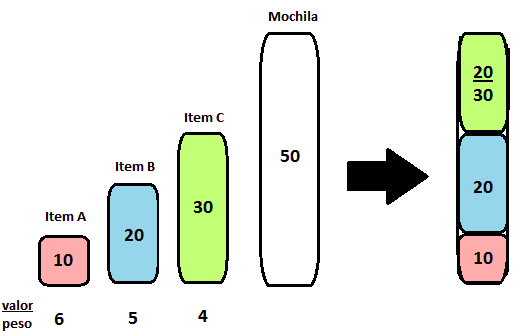
\includegraphics[keepaspectratio=true,scale=0.5]{figuras/mochila.png}
\caption{Problema da mochila fracionária - Algoritmo Guloso}
\label{mochila}
\end{figure}

E para a mochila binária, o valor máximo alcançado seria de 160, como mostra a Figura \ref{mochilabinaria}.

\FloatBarrier
\begin{figure}[!h]
\centering
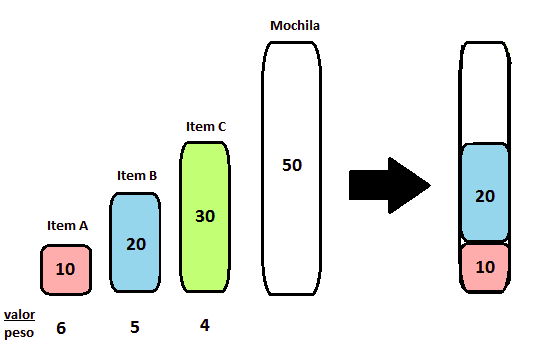
\includegraphics[keepaspectratio=true,scale=0.5]{figuras/mochilabinaria.png}
\caption{Problema da mochila binária - Algoritmo Guloso}
\label{mochilabinaria}
\end{figure}

Como é possível perceber, na resolução da mochila binária, o algoritmo guloso não obtém sucesso, uma vez que a melhor solução teria o valor máximo igual 220, como demonstra a Figura \ref{mochilabinariacerta}.
\clearpage 

\FloatBarrier
\begin{figure}[!h]
\centering
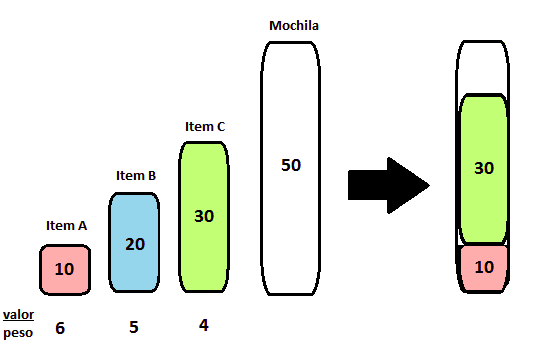
\includegraphics[keepaspectratio=true,scale=0.5]{figuras/mochilabinariacerta.png}
\caption{Problema da mochila binária - Resposta}
\label{mochilabinariacerta}
\end{figure}

\item \textbf{Resolução por programação dinâmica:} Na resolução da mochila binária por programação dinâmica, é criada uma matriz onde as linhas são os itens e cada coluna representa a capacidade da mochila ordenada de forma crescente. No caso do exemplo anteriormente citado, seria criada uma matriz igual a mostrada na Figura \ref{matriz}.

\FloatBarrier
\begin{figure}[!h]
\centering
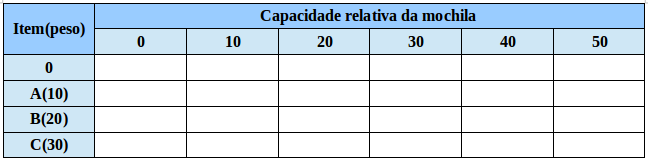
\includegraphics[keepaspectratio=true,scale=0.5]{figuras/matriz.png}
\caption{Problema da mochila binária - Programação Dinâmica}
\label{matriz}
\end{figure}

A análise se inicia na primeira célula (linha 1, coluna 1), e a cada passo vai analisando a próxima célula da linha, quando chega ao final, volta à primeira coluna e desce para a segunda linha, caracterizando uma análise \textit{top-down}. 

A cada iteração, é analisado primeiramente o peso do item em relação a capacidade relativa da mochila (referente a coluna que se está analisando), podendo resultar em três cenários: 
\begin{enumerate}
\item \textbf{Peso analisado é igual à capacidade relativa:} nesse cenário, o algoritmo pergunta a si próprio: O que é melhor? Tomar o valor da célula anterior, tomar o valor da célula acima ou tomar o valor do item analisado? Após a decisão, o algoritmo grava o valor na matriz.
\item \textbf{Peso analisado é inferior à capacidade relativa:} nesse cenário, o algoritmo pergunta a si próprio: É melhor tomar o valor da célula acima ou é melhor tomar o valor do item analisado somado à célula da linha acima que complemente o peso analisado, de forma que a capacidade relativa seja alcançada? Após tomada a decisão, o algoritmo grava o valor na matriz. 
\item \textbf{Peso analisado é superior à capacidade relativa:} nesse cenário, não é possível tomar o valor do item analisado. Logo, o algoritmo pergunta a si próprio: é melhor tomar o valor da célula ao lado ou da célula acima? 
\end{enumerate}

Dada uma matriz (NxM), a última célula da mesma (linha N, coluna M) contém a resposta para o problema analisado. 

Tomando como exemplo a Tabela \ref{knapsack}, a solução por programação dinâmica cria uma matriz como a da Figura \ref{matriz} e preenche a primeira linha e a primeira coluna com zeros, como mostra a Figura \ref{matrizZero}, pois se a capacidade da mochila é zero (primeira coluna) não tem como pegar item. Como não tem item para analisar (primeira linha), não tem como tomar valor algum. Mesmo na prática não existindo uma mochila sem capacidade ou nenhum item para ser analisado, essas hipóteses são acrescentadas para que na hora da execução do algoritmo não ocorra erro, já que o algoritmo está sempre analisando o valor de outras células para a tomada de decisão.

\FloatBarrier
\begin{figure}[!h]
\centering
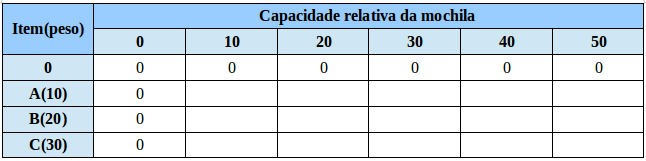
\includegraphics[keepaspectratio=true,scale=0.5]{figuras/matrizZero.png}
\caption{Problema da mochila binária - PD - Passo Inicial}
\label{matrizZero}
\end{figure}

O segundo passo é analisar a capacidade da mochila sendo 10, e havendo apenas o item A, com peso 10. Logo, tem-se o cenário do peso analisado igual à capacidade relativa, e obviamente, o melhor, nesse caso, é tomar o valor do item analisado, ou seja, escrever 60 na célula, como mostra a Figura \ref{matriz60}.

\FloatBarrier
\begin{figure}[!h]
\centering
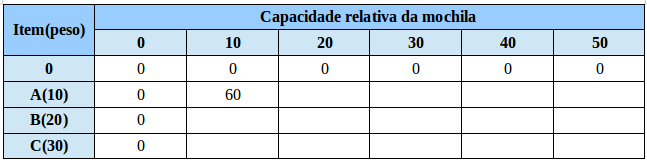
\includegraphics[keepaspectratio=true,scale=0.5]{figuras/matriz60.png}
\caption{Problema da mochila binária - PD - Item A, Capacidade 10}
\label{matriz60}
\end{figure}

Em seguida, é analisada a capacidade da mochila como sendo 20. Nesse casso, existe apenas o item A, de peso 10, para ser colocado na mochila. Imediatamente é percebido, por nós humanos, que o valor desse item será escrito na célula. Porém, a progração dinâmica não tem esse conhecimento, e avalia o cenário de peso analisado inferior à capacidade relativa da mochila. Nesse cenário, é possível tomar o valor da célula acima, que é zero, ou o valor do item de peso 10 somado ao seu complemento, contido na linha acima, que o faz alcançar a capacidade da mochila. A coluna que complementa o peso do item é a de valor 10, pois assim é alcançado o valor 20 da capacidade relativa analisada. As Figuras \ref{matriz10_20} e \ref{matriz10_20_resp} demonstram essa decisão.

\FloatBarrier
\begin{figure}[!h]
\centering
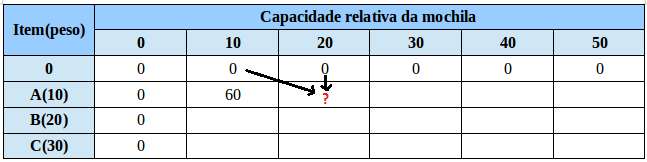
\includegraphics[keepaspectratio=true,scale=0.6]{figuras/matriz10_20.png}
\caption{Problema da mochila binária - PD - Item A, Capacidade 20 - Análise }
\label{matriz10_20}
\end{figure}

\FloatBarrier
\begin{figure}[!h]
\centering
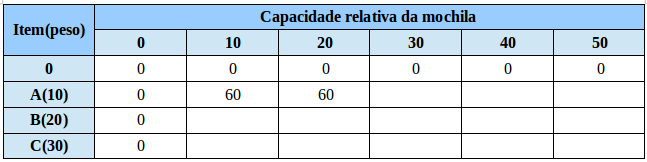
\includegraphics[keepaspectratio=true,scale=0.6]{figuras/matriz10_20_resp.png}
\caption{Problema da mochila binária - PD - Item A, Capacidade 20 - Resultado}
\label{matriz10_20_resp}
\end{figure}

Essa análise é feita para toda a linha, como mostram as Figuras \ref{matriz10_30}, \ref{matriz10_30_resp}, \ref{matriz10_40}, \ref{matriz10_40_resp}, \ref{matriz10_50} e \ref{matriz10_50_resp}, onde em todos os passos foi decidido, pela programação dinâmica, a soma do valor do item A, que é 60, e o seu complemento, que em todos os casos tem valor zero.

\FloatBarrier
\begin{figure}[!h]
\centering
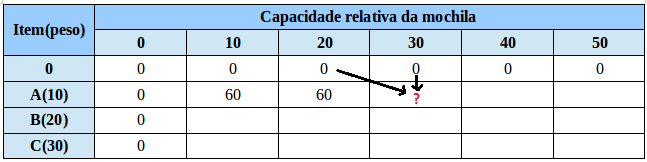
\includegraphics[keepaspectratio=true,scale=0.6]{figuras/matriz10_30.png}
\caption{Problema da mochila binária - PD - Item A, Capacidade 30 - Análise}
\label{matriz10_30}
\end{figure}

\FloatBarrier
\begin{figure}[!h]
\centering
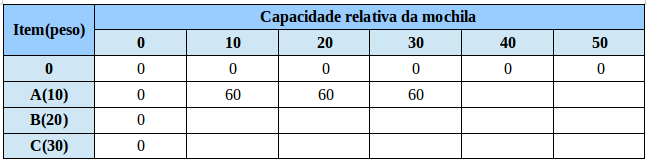
\includegraphics[keepaspectratio=true,scale=0.6]{figuras/matriz10_30_resp.png}
\caption{Problema da mochila binária - PD - Item A, Capacidade 30 - Resultado}
\label{matriz10_30_resp}
\end{figure} 

\FloatBarrier
\begin{figure}[!h]
\centering
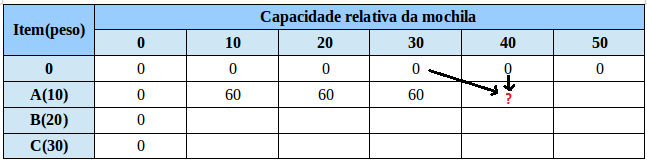
\includegraphics[keepaspectratio=true,scale=0.6]{figuras/matriz10_40.png}
\caption{Problema da mochila binária - PD - Item A, Capacidade 40 - Análise}
\label{matriz10_40}
\end{figure}

\FloatBarrier
\begin{figure}[!h]
\centering
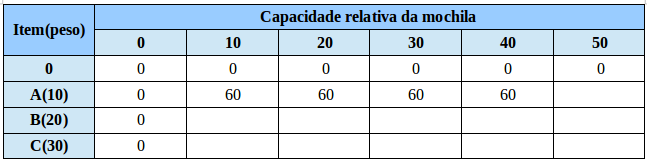
\includegraphics[keepaspectratio=true,scale=0.6]{figuras/matriz10_40_resp.png}
\caption{Problema da mochila binária - PD - Item A, Capacidade 40 - Resultado}
\label{matriz10_40_resp}
\end{figure}

\FloatBarrier
\begin{figure}[!h]
\centering
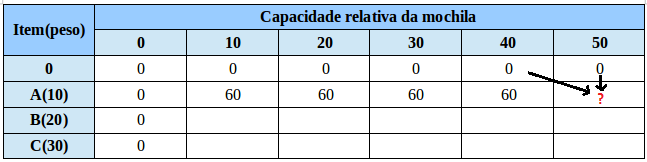
\includegraphics[keepaspectratio=true,scale=0.6]{figuras/matriz10_50.png}
\caption{Problema da mochila binária - PD - Item A, Capacidade 50 - Análise}
\label{matriz10_50}
\end{figure}

\FloatBarrier
\begin{figure}[!h]
\centering
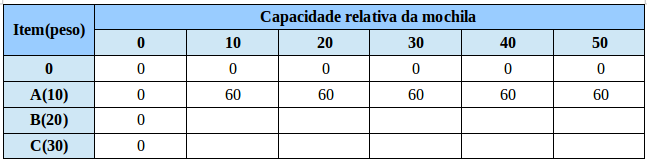
\includegraphics[keepaspectratio=true,scale=0.6]{figuras/matriz10_50_resp.png}
\caption{Problema da mochila binária - PD - Item A, Capacidade 50 - Resultado}
\label{matriz10_50_resp}
\end{figure}
 
A análise do item B, de peso 20, quando a capacidade da mochila é 10, é o cenário de peso analisado superior à capacidade relativa. Nesse caso, é possível continuar com o valor contindo na mochila na capacidade relativa anterior (célula anterior), ou pode-se tomar o valor do item anterior quando a capacidade relativa da mochila é a mesma (célula acima). Dessa forma, a programação dinâmica decide pela célula acima e escreve seu valor na célula analisada. As Figuras \ref{matriz20_10} e \ref{mochila20_10_resp} demonstram essa decisão.

\FloatBarrier
\begin{figure}[!h]
\centering
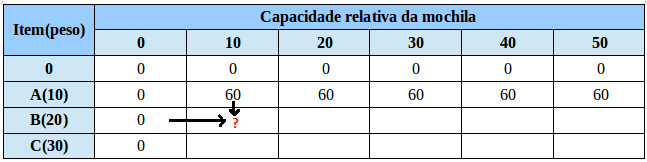
\includegraphics[keepaspectratio=true,scale=0.5]{figuras/matriz20_10.png}
\caption{Problema da mochila binária - PD - Item B, Capacidade 10 - Análise}
\label{matriz20_10}
\end{figure}

\FloatBarrier
\begin{figure}[!h]
\centering
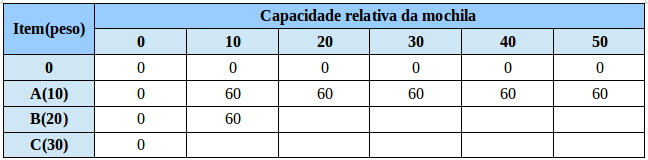
\includegraphics[keepaspectratio=true,scale=0.5]{figuras/mochila20_10_resp.png}
\caption{Problema da mochila binária - PD - Item B, Capacidade 10 - Resultado}
\label{mochila20_10_resp}
\end{figure}

As demais decisões são efetuadas seguindo um dos passo-a-passo anteriormente citados, dependendo do cenário que se está analisando. As Figuras \ref{mochila20_20}, \ref{mochila20_20_resp}, \ref{mochila20_30}, \ref{mochila20_30_resp}, \ref{mochila20_40}, \ref{mochila20_40_resp}, \ref{mochila20_50}, \ref{mochila20_50_resp}, \ref{mochila30_10}, \ref{mochila30_10_resp}, \ref{mochila30_20}, \ref{mochila30_20_resp}, \ref{mochila30_30}, \ref{mochila30_30_resp}, \ref{mochila30_40}, \ref{mochila30_40_resp}, \ref{mochila30_50} e \ref{mochila30_50_resp} demonstram tais decisões.
\FloatBarrier
\begin{figure}[!h]
\centering
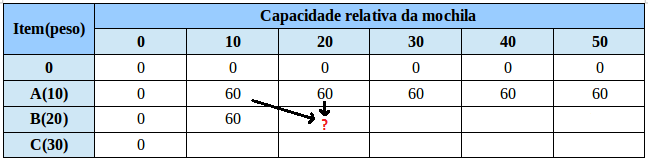
\includegraphics[keepaspectratio=true,scale=0.6]{figuras/mochila20_20.png}
\caption{Problema da mochila binária - PD - Item B, Capacidade 20 - Análise}
\label{mochila20_20}
\end{figure}

\FloatBarrier
\begin{figure}[!h]
\centering
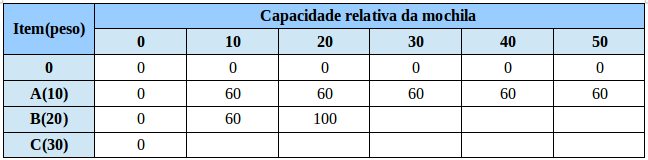
\includegraphics[keepaspectratio=true,scale=0.6]{figuras/mochila20_20_resp.png}
\caption{Problema da mochila binária - PD - Item B, Capacidade 20 - Resultado}
\label{mochila20_20_resp}
\end{figure}

\FloatBarrier
\begin{figure}[!h]
\centering
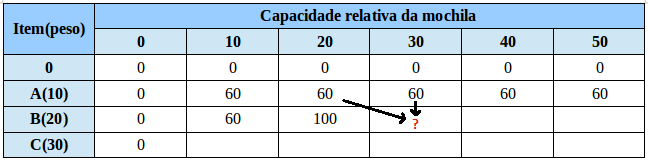
\includegraphics[keepaspectratio=true,scale=0.6]{figuras/mochila20_30.png}
\caption{Problema da mochila binária - PD - Item B, Capacidade 30 - Análise}
\label{mochila20_30}
\end{figure}

\FloatBarrier
\begin{figure}[!h]
\centering
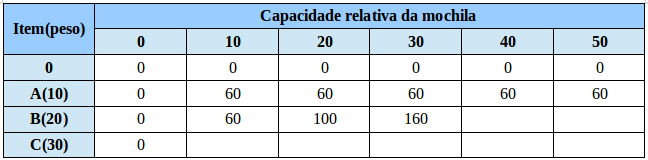
\includegraphics[keepaspectratio=true,scale=0.6]{figuras/mochila20_30_resp.png}
\caption{Problema da mochila binária - PD - Item B, Capacidade 30 - Resultado}
\label{mochila20_30_resp}
\end{figure}

\FloatBarrier
\begin{figure}[!h]
\centering
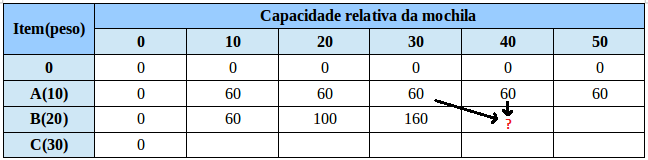
\includegraphics[keepaspectratio=true,scale=0.6]{figuras/mochila20_40.png}
\caption{Problema da mochila binária - PD - Item B, Capacidade 40 - Análise}
\label{mochila20_40}
\end{figure}

\FloatBarrier
\begin{figure}[!h]
\centering
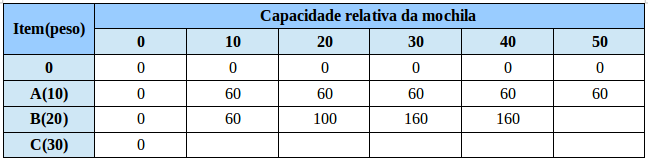
\includegraphics[keepaspectratio=true,scale=0.6]{figuras/mochila20_40_resp.png}
\caption{Problema da mochila binária - PD - Item B, Capacidade 40 - Resultado}
\label{mochila20_40_resp}
\end{figure}

\FloatBarrier
\begin{figure}[!h]
\centering
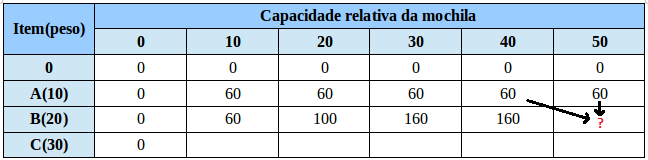
\includegraphics[keepaspectratio=true,scale=0.6]{figuras/mochila20_50.png}
\caption{Problema da mochila binária - PD - Item B, Capacidade 50 - Análise}
\label{mochila20_50}
\end{figure}

\FloatBarrier
\begin{figure}[!h]
\centering
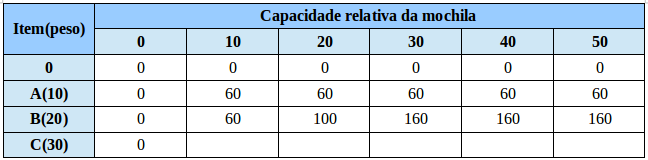
\includegraphics[keepaspectratio=true,scale=0.6]{figuras/mochila20_50_resp.png}
\caption{Problema da mochila binária - PD - Item B, Capacidade 50 - Resultado}
\label{mochila20_50_resp}
\end{figure}

\FloatBarrier
\begin{figure}[!h]
\centering
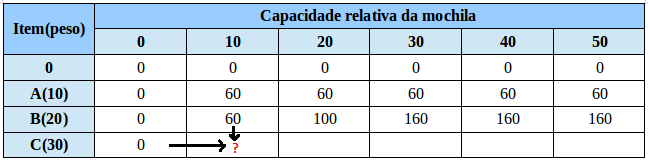
\includegraphics[keepaspectratio=true,scale=0.6]{figuras/mochila30_10.png}
\caption{Problema da mochila binária - PD - Item C, Capacidade 10 - Análise}
\label{mochila30_10}
\end{figure}

\FloatBarrier
\begin{figure}[!h]
\centering
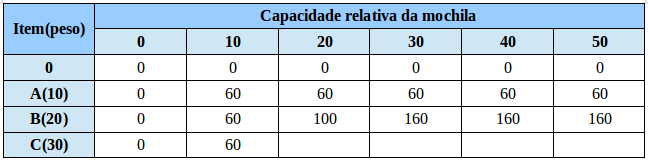
\includegraphics[keepaspectratio=true,scale=0.6]{figuras/mochila30_10_resp.png}
\caption{Problema da mochila binária - PD - Item C, Capacidade 10 - Resultado}
\label{mochila30_10_resp}
\end{figure}

\FloatBarrier
\begin{figure}[!h]
\centering
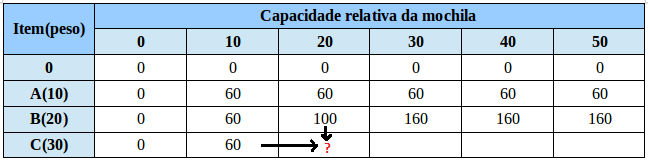
\includegraphics[keepaspectratio=true,scale=0.6]{figuras/mochila30_20.png}
\caption{Problema da mochila binária - PD - Item C, Capacidade 20 - Análise}
\label{mochila30_20}
\end{figure}

\FloatBarrier
\begin{figure}[!h]
\centering
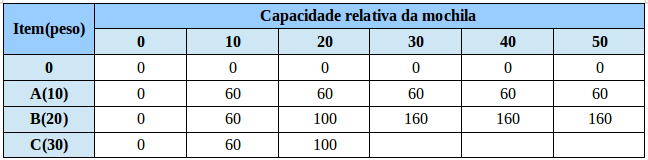
\includegraphics[keepaspectratio=true,scale=0.6]{figuras/mochila30_20_resp.png}
\caption{Problema da mochila binária - PD - Item C, Capacidade 20 - Resultado}
\label{mochila30_20_resp}
\end{figure}

As Figuras \ref{mochila30_30} e \ref{mochila30_30_resp} mostram a decisão da programação dinâmica quando um cenário de peso analisado é igual a capacidade relativa da mochila, onde a melhor opção foi não foi tomar o valor do item, que seria 120, mas tomar o valor do item anterior na mesma capacidade relativa (célula acima), que é 160.
\FloatBarrier
\begin{figure}[!h]
\centering
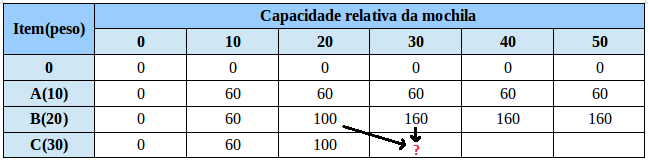
\includegraphics[keepaspectratio=true,scale=0.6]{figuras/mochila30_30.png}
\caption{Problema da mochila binária - PD - Item C, Capacidade 30 - Análise}
\label{mochila30_30}
\end{figure}

\FloatBarrier
\begin{figure}[!h]
\centering
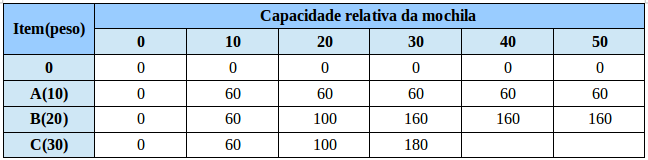
\includegraphics[keepaspectratio=true,scale=0.6]{figuras/mochila30_30_resp.png}
\caption{Problema da mochila binária - PD - Item C, Capacidade 30 - Resultado}
\label{mochila30_30_resp}
\end{figure}

\FloatBarrier
\begin{figure}[!h]
\centering
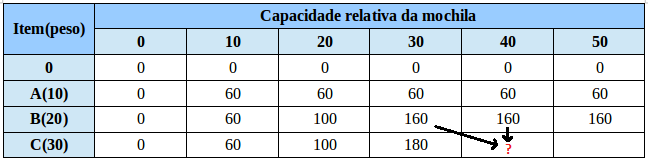
\includegraphics[keepaspectratio=true,scale=0.6]{figuras/mochila30_40.png}
\caption{Problema da mochila binária - PD - Item C, Capacidade 40 - Análise}
\label{mochila30_40}
\end{figure}

\FloatBarrier
\begin{figure}[!h]
\centering
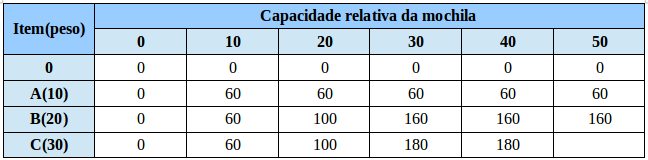
\includegraphics[keepaspectratio=true,scale=0.6]{figuras/mochila30_40_resp.png}
\caption{Problema da mochila binária - PD - Item C, Capacidade 40 - Resultado}
\label{mochila30_40_resp}
\end{figure}

\FloatBarrier
\begin{figure}[!h]
\centering
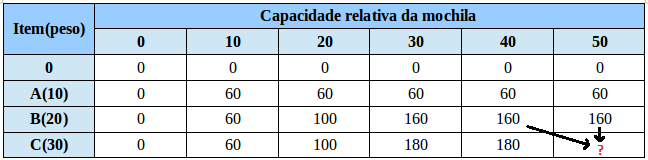
\includegraphics[keepaspectratio=true,scale=0.6]{figuras/mochila30_50.png}
\caption{Problema da mochila binária - PD - Item C, Capacidade 50 - Análise}
\label{mochila30_50}
\end{figure}

\FloatBarrier
\begin{figure}[!h]
\centering
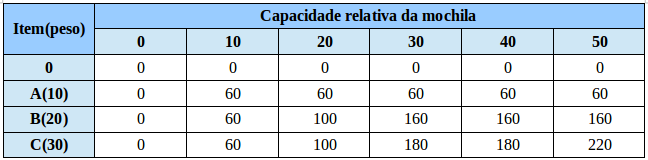
\includegraphics[keepaspectratio=true,scale=0.5]{figuras/mochilaResultado.png}
\caption{Problema da mochila binária - PD - Item C, Capacidade 50 - Resultado}
\label{mochila30_50_resp}
\end{figure}

O valor da última célula é a resposta para o problema. Como é possível ver na Figura \ref{mochila30_50_resp}, o valor encontrado pela programação dinâmica foi 220, demonstrando que para o problema da mochila binária, o algoritmo é eficaz.
\end{itemize}
 
\subsubsection{Adaptação do problema da mochila para o contexto do trabalho}
Para o completo entendimento do trabalho proposto, algumas definições sobre termos amplamente utilizados no kit LEGO Mindstorms NXT se fazem necessárias e são feitas a seguir.
\begin{itemize}
\item \textbf{Missão:} uma missão é composta por uma tarefa que deve ser executada pelo robô em um determinado tempo, valendo uma pontuação, e por um trajeto que deve ser efetuado pelo robô para executar a missão;
\item \textbf{Pontuação da missão:} cada missão tem uma pontuação previamente estabelecida. Essa pontuação é alcançada se a missão for concluída com sucesso;
\item \textbf{Pontuação total:} é o somatório das pontuações de todas as missões concluídas com sucesso;
\item \textbf{Mapa:} um mapa é onde o robô deve executar as missões. Cada mapa contém diferentes missões associados a ele;
\item \textbf{Tempo total:} é uma quantidade de tempo, previamente estabelecida, geralmente de dois a três minutos, utilizada para executar o máximo de missões possíveis almejando a maior pontuação total;
\item \textbf{Tempo restante:} é a quantidade de tempo que falta para chegar ao fim do tempo total;
\item \textbf{Tempo da tarefa:}  é a quantidade de tempo necessária para que o robô execute uma tarefa;
\item \textbf{Tempo do trajeto:} é a quantidade de tempo que o robô utiliza para chegar em um local com coordenadas (X, Y) partindo de um local com coordenadas (X0, Y0);
\item \textbf{Tempo da missão:} é a quantidade de tempo utilizada para concluir a missão com sucesso.
\item \textbf{Base:} local no mapa de onde o robô deve partir para executar a primeira missão. 
\end{itemize}

O objetivo do trabalho é alcançar a maior pontuação dentro de um determinado espaço de tempo. Supondo que existam três missões para o robô executar, missão da árvore, missão dos pets e missão do avião, descritas a seguir, quais missões devem ser executadas, dentro de um tempo restante de 50 segundos, para se alcançar a maior pontuação?

\begin{itemize}
\item \textbf{Missão árvore:} Essa missão consiste de uma tarefa em que o robô tem que derrubar o galho de uma árvore, sem deixar que ele encoste nos fios de alta tensão. Tempo de execução da tarefa: 5 segundos; Tempo da trajetória: 5 segundos; Tempo da missão: Tempo da trajetória + tempo da tarefa = 10 segundos;
\item \textbf{Missão pets:} Essa missão consiste na tarefa de resgatar os pets e levá-los à base. Tempo de execução da tarefa: 10 segundos; Tempo da trajetória: 10 segundos; Tempo da missão: 20 segundos;
\item \textbf{Missão avião}: Essa missão consiste na tarefa de derrubar o avião na pista de pouso. Tempo de execução da tarefa: 10 segundos; Tempo da trajetória: 20 segundos; Tempo de execução da missão: 20 segundos;
\end{itemize}

Da mesma forma que no problema da mochila binária não é possível pegar uma fração de um objeto, no contexto desse trabalho não é possível executar uma fração de uma missão, tornando o problema binário para ganhar a pontuação da missão. Desta forma, é criada uma matriz onde o eixo X é o tempo restante e o eixo Y é o tempo de execução de cada missão, como mostra a Figura \ref{matrizProlego}.

\FloatBarrier
\begin{figure}[!h]
\centering
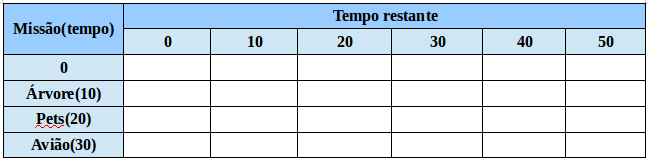
\includegraphics[keepaspectratio=true,scale=0.6]{figuras/matrizProlego.png}
\caption{Prolego - Programação Dinâmica}
\label{matrizProlego}
\end{figure}


Resolvendo essa matriz com programação dinâmica é alcançado o valor de 220, como mostra a Figura \ref{matrizProlegoResult}, ou seja, as missões que devem ser executadas são: missão pets e missão avião.  

\FloatBarrier
\begin{figure}[!h]
\centering
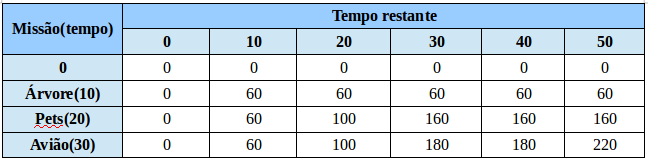
\includegraphics[keepaspectratio=true,scale=0.6]{figuras/matrizProlegoResult.png}
\caption{Prolego - Programação Dinâmica - Resultado}
\label{matrizProlegoResult}
\end{figure}

\section{Considerações parciais}
Este trabalho propõe uma implementação de um algoritmo de programação dinâmica que otimize a execução de missões pelo robô, afim de aproveitar melhor o tempo restante para conseguir a maior pontuação possível. Trata-se de uma pesquisa híbrida exploratória/experimental para o levantamento da solução da questão de pesquisa, e exploratória-descritiva para construção do algoritmo. 
A fim de refinar a proposta inicial do trabalho, que antes era baseada apenas no referencial teórico estudado, foi elaborada uma prova de conceito, avaliando três ferramentas candidatas para a integração do robô com o Prolog. Adicionalmente, comparou-se  o algoritmo guloso e a programação dinâmica com o propósito de demonstrar as razões pelas quais a programação dinâmica foi selecionada para ser utilizada nesse trabalho.
Com a avaliação das ferramentas candidatas foi possível perceber alguns problemas em relação a cada uma delas. Alguns problemas se mostraram mais graves que outros, o que inviabilizou a utilização de duas ferramentas, elegendo assim a ferramenta PLNXT, a qual será utilizada nesse trabalho.